%!TEX TS-options = --shell-escape
%!TEX TS-program = pdflatex
\documentclass[%
   10pt,              % Schriftgroesse
                 % wird an andere Pakete weitergereicht
   a4paper,           % Seitengroesse
   DIV10,             % Textbereichsgroesse (siehe Koma Skript Dokumentation !)
]{scrartcl}%     Klassen: scrartcl, scrreprt, scrbook, article
% -------------------------------------------------------------------------

\usepackage[utf8]{inputenc} % Font Encoding, benoetigt fuer Umlaute
%\usepackage[ngerman]{babel}   % Spracheinstellung


\usepackage{ulem}
\usepackage{graphicx}
\usepackage{amsfonts}
\usepackage{amsmath}
\usepackage{hyperref}
\usepackage{enumitem}
\usepackage{tikz}
\usepackage{multirow}
\usepackage{listings}
\usepackage{ifthen}
\usepackage{todonotes}
\usetikzlibrary{automata,arrows}
\usepackage{pgfplots}
\usepackage{booktabs}


% Definition des Headers
\usepackage{geometry}
\geometry{a4paper, top=3cm, left=3cm, right=3cm, bottom=3cm, headsep=0mm, footskip=0mm}
\renewcommand{\baselinestretch}{1.3}\normalsize
%\renewcommand{\labelenumi}{\alph{enumi})}
\newcommand{\norm}[1]{\left\lVert#1\right\rVert}
\def\header#1#2#3#4#5#6{\pagestyle{empty}
\noindent
\begin{minipage}[t]{0.6\textwidth}
\begin{flushleft}
\textbf{#4}\\% Fach
#6\\% Semester
#2  % Tutor 
\end{flushleft}
\end{minipage}
\begin{minipage}[t]{0.4\textwidth}
\begin{flushright}
\vspace*{0.2cm}
#5%  Names
\end{flushright}
\end{minipage}

\begin{center}
{\Large\textbf{ #1}} % Blatt

{(#3)} % Abgabedatum
\end{center}
}

\newenvironment{vartab}[1]
{
    \begin{tabular}{ |c@{} *{#1}{c|} } %\hline
}{
    \end{tabular}
}

\newcommand{\myformat}[1]{& #1}

\newcommand{\entry}[1]{
  \edef\result{\csvloop[\myformat]{#1}}
  \result \\ \hline
}

\newcommand{\numbers}[1]{
  \newcounter{ctra}
\setcounter{ctra}{1}
\whiledo {\value{ctra} < #1}%
{%
  \myformat{\thectra}
  \stepcounter{ctra}%
}
\myformat{\thectra}
}
\newcommand{\emptyLine}[1]{
  \newcounter{ctra1}
\setcounter{ctra}{1}
\whiledo {\value{ctra1} < #1}%
{%
  \myformat{\hspace*{0.5cm}}
  \stepcounter{ctra1}%
}
}

\begin{document}
%\header{Blatt}{Tutor}{Abgabedatum}{Vorlesung}{Bearbeiter}{Semester}{Anzahl Aufgaben}
\header{Skin Cancer Detection}{Prof. Schilling}{28. November 2017}{Praktikum Maschinelles Lernen}{Florence Lopez \\ Jonas Einig \\ Julian Späth}{WS 17/18}

\section*{Beschreibung}

 \begin{figure}[ht]
	\centering
 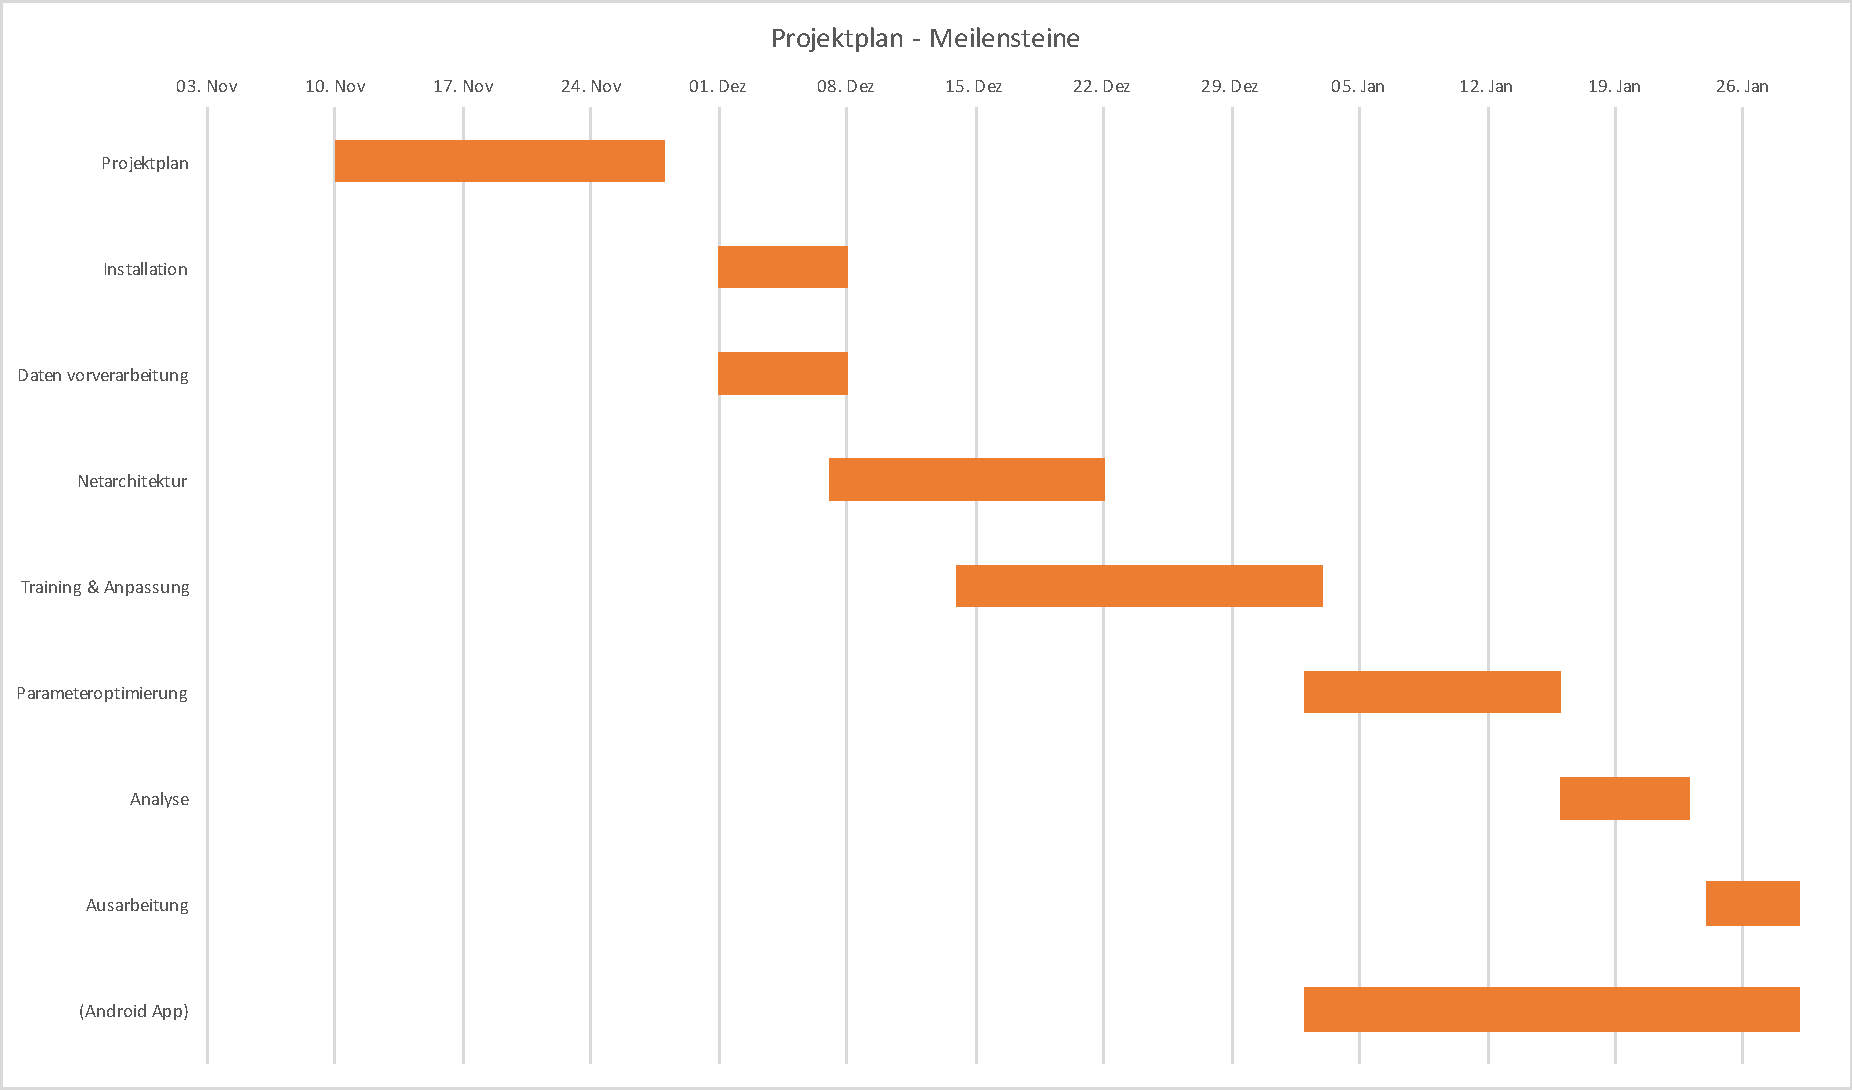
\includegraphics[width=\textwidth]{fig/gantt_projektplan}
 \caption{Meilensteine des Projekts als GANTT-Chart}
	\label{fig_gantt}
 \end{figure}

\section*{Tools}

\section*{Daten}

\section*{Methode}

\section*{Optional: Android App}

\section*{Kontakt}
\centering
\begin{tabular}{lll}
\toprule
Name & Matrikelnummer & E-Mail Adresse \\
\midrule
Florence Lopez & XXXXXXX  &  \href{mailto:florence.lopez@student.uni-tuebingen.de}{florence.lopez@student.uni-tuebingen.de} \\
Jonas Einig  & XXXXXXX    & \href{mailto:jonas.einig@student.uni-tuebingen.de}{jonas.einig@student.uni-tuebingen.de}    \\
Julian Späth  & 3938726    & \href{mailto:julian.spaeth@student.uni-tuebingen.de}{julian.spaeth@student.uni-tuebingen.de}    \\
\bottomrule
\end{tabular}


\end{document}